\section{Considerações Iniciais}\label{sec:consideracoes_iniciais}
Geralmente refatorações são aplicadas para melhorar a qualidade do software (por exemplo, a extensibilidade, a modularidade, a capacidade de reutilização, a complexidade, manutenção, etc). 
A maioria das pesquisas apontam que usualmente refatorações são aplicadas em nível de código-fonte~\cite{Fowler1999, Demeyer1, Demeyer2, Opdy92b}. Tais pesquisas não estão preocupadas em como promover o reuso e o compartilhamento de refatorações e também não estão interessadas e criar refatorações para outros tipos de artefatos, tais como os artefatos providos pela ADM, por exemplo, o metamodelo KDM. 
%
Como já destacado, na literatura é possível identificar um conjunto de refatorações já validadas e que são usualmente aplicadas em código-fonte, por exemplo, \textit{Extract Class}, \textit{Move Method}, \textit{Move Attribute}, etc. Essas são apenas alguns exemplos de refatorações úteis que não são facilmente reutilizadas na prática durante a condução de modernização de um determinado sistema. Essa limitação pode ser atribuída devido a ausência de um meio padronizado de disponibilizar refatorações. 
Uma abordagem promissora é lidar com a refatoração de forma independente da linguagem – aumentando assim as possibilidades de reutilização de refatorações.

Como ressaltado no Capítulo~\ref{chapter:adm_kdm} a ADM fornece um conjunto de metamodelos para auxiliar o engenheiro de software a conduzir MDRE. 
Porém, até esse momento a ADM não provê instruções ou ate mesmo um metamodelo para auxiliar o engenheiro a promover o reuso de refatorações juntamente com os seus metamodelos padronizados (por exemplo, KDM) durante o processo de modernização. 
Essa limitação faz com que o engenheiro crie suas próprias soluções/refatorações, resultando em um possível atraso no processo de modernização. 
Além disso, no Capítulo~\ref{chapter:catalogo_refactoring_KDM} é apresentado um catalogo de refatorações dedicado para o metamodelo KDM que se baseia no catálogo proposto for Fowler~\cite{Fowler1999}. Contudo, as refatorações definidas não podem ser facilmente reutilizadas e compartilhadas entre os modernizadores. 
Com o intuito de suprir tal limitação neste capítulo é apresentado um metamodelo para auxiliar o engenheiro a promover o reuso de refatorações no contexto do metamodelo KDM. Com a utilização desse metamodelo, informações (metadados) sobre refatorações podem ser reutilizadas de forma independente de linguagem e plataforma. 

É importante ressaltar que esse metamodelo foi criado para promover reuso de refatorações. Além disso, o metamodelo aqui proposto tem as seguintes características: (\textit{i}) é um metamodelo de refatoração que permite a interoperabilidade de refatorações para um amplo domínio e (\textit{ii}) auxilia o engenheiro de modernização à definir refatorações representativas em forma de metadados. Nota-se que o metamodelo aqui proposto é totalmente integrado com o metamodelo KDM. Em outras palavras, uma instância do metamodelo de refatoração contêm metadados de um refatoração escrita para ser aplicado em uma instância do metamodelo KDM. A escolha do metamodelo KDM se deu pois o mesmo é um metamodelo padronizado pela OMG, além de ser um metamodelo PIM, o que significa que quaisquer refatorações aplicadas em uma instância do KDM, podem ser consideradas independentes de linguagem e de plataforma e então ser transformado para em um PSM (ver Capítulo~\ref{chapter:fundamentacao_teorica} e Capítulo\ref{chapter:adm_kdm}). Utilizar refatorações como um metamodelo (de forma independente de linguagem) pode abrir opções para promover a reutilização de refatorações. Por exemplo, dado uma instância do metamodelo de refatoração, o engenheiro de software poderia utilizar essa instância para aplicar a refatoração em qualquer sistema representado pelo KDM. Além disso, um determinado engenheiro de software poderia instanciar o metamodelo de refatoração, criar um catalogo de refatorações e disponibilizar para que outros possam reutilizar tais refatorações. Tornando assim possível o compartilhamento e o reuso de refatorações no contexto da ADM.

Com o intuito de apresentar o metamodelo de uma maneira mais prática, neste capítulo a construção do mesmo é realizado com o uso do EMF~\cite{EMF}. Porém, ressalta-se que o metamodelo pode ser criado com o uso de outras tecnologias.

As demais seções deste capítulo estão organizadas da seguinte forma: na Seção.... é apresentada a motivação para a criação do metamodelo de refatoração; na Seção ... o metamodelo é apresentado..., na Seção .. são feitas as considerações finais a respeito do metamodelo de refatoração proposto neste capítulo.

\section{Motivação para a criação de um metamodelo de refatoração} % (fold)
\label{sec:motiva_o_para_a_cria_o_de_um_meta_modelo_de_refatora_o}

Durante o mapeamento sistemático conduzido (ver Capítulo~\ref{chapter:mapeamento_sistematico})~\cite{durelli_systematic_mapping} pôde-se observar na literatura a carência de estudos que definem soluções para especificar e promover o reuso de refatorações no contexto da ADM e do metamodelo KDM. Sem a adequada representação de refatorações para o KDM, a especificação e realização de uma refatoração pode se tornar uma atividade propensa a erros e difícil de reutilizar.

Neste contexto, suponha o seguinte cenário, um engenheiro define uma determinada refatoração e a compartilha por meio de um repositório. Dessa forma, outros engenheiros podem então navegador nesse repositório e identificar, não apenas essa, mas um conjunto de refatorações. O engenheiro então escolhe uma determinada refatoração no repositório, faz o \textit{download} e a reutiliza em seu sistema representado em nível de uma instância do metamodelo KDM. 

Uma das soluções para a concretização desse cenário seria a criação de um metamodelo para persistir metadados relacionados com refatorações. Esse metamodelo deveria então contêm metaclasses para armazenar metadados importantes de uma específica refatoração, por exemplo, o nome da refatoração, sua motivação, os passos para sua realização, e até mesmo o mecanismo e sua pré- e pós-condições. Como ressaltado anteriormente, devido a carência de um metamodelo que possui tais características, esse capítulo têm como principal objetivo definir um metamodelo que permita a representação de meta-informações relacionadas com refatorações, porém, ainda respeite e siga as diretrizes dos metamodelos definidos na abordagem ADM, por exemplo, o metamodelo aqui definido precisa ser independente de linguagem e plataforma.

Essa ultima características é de suma importância, assim, o metamodelo aqui apresentado é baseado nas metaclasses do KDM. Em outras palavras, uma instância desse metamodelo de refatoração, deve conter referencias a novas metaclasses específicas para definir metadados sobre refatorações e também intâncias das metaclasses do KDM, tornando assim, a operação/mecanismo de uma refatoração independente de plataforma e linguagem de programação. Dessa forma, o metamodelo pode então ser facilmente utilizado e aplicado em ferramentas existentes que utilizam como base o KDM aumentando a interoperabilidade de futuras ferramentas que utilizem esse metamodelo de refatoração. Levando em consideração as motivações destacadas, na Seção~\ref{sec:meta_modelo_de_refatora_es_estruturadas_srm_do_ingl_s_structured refactoring meta-model_} é apresentado o metamodelo de refatorações estruturadas (do inglês - Structured Refactoring Metamodel – SRM).  


%Além disso, uma característica de suma importância é que esse metamodelo de refatoração seja baseado nas metaclasses do KDM. Em outras palavras, uma instancia desse metamodelo, deve conter referencias a metaclasses do KDM, tornando assim, a operação/mecanismo de um refatoração independente de plataforma e linguagem. 

\section{Metamodelo de Refatorações Estruturadas} % (fold)
\label{sec:meta_modelo_de_refatora_es_estruturadas_srm_do_ingl_s_structured refactoring meta-model_}

Como pôde ser observado na seção anterior, são várias as motivações para a definição de um metamodelo para especificar refatorações. Neste sentido, nesta seção é apresentado o metamodelo de Refatorações Estruturadas (do inglês - \sigla{SRM}{Structured Refactoring Metamodel})

Refatorações são ubíquas durante a manutenção, produção, análise de software. Inúmeras comunidades têm surgido na literatura para criar e definir vários tipos de refatorações, incluindo refatorações de baixa granularidade~\cite{Fowler1999, Demeyer1, Demeyer2}, refatorações arquiteturais, refatorações para o paradigma orientado a aspecto, etc. Neste contexto, há uma grande necessidade da definição de um padrão para auxiliar e promover o compartilhamento dessas refatorações, tanto dentro como entre estas comunidades. Assim, esta seção descreve e define um metamodelo para auxiliar tais comunidades, para apoiar vários casos de uso de refatorações e também para facilitar a iterações entre os desenvolvedores de refatorações. Esse metamodelo cria e representa uma fundamentação para o compartilhamento de informações (metadados) relacionadas com refatorações, assim, detalhes com informações precisas sobre uma especifica refatoração pode ser armazenada e compartilhada para que outros engenheiros possam reutilizar em seus projetos que utilizem o metamodelo KDM.

Por exemplo, uma comunidade que cria refatorações de baixa granularidade usualmente esta preocupada em definir e especificar refatorações desse tipo. Por outro lado, uma comunidade que especifica refatorações arquiteturais esta interessada apenas em refatoração arquiteturais. Porém, nota-se que ambas comunidades têm em comum a necessidade de especificar como organizar e definir as refatorações. Além disso, tais comunidades devem se preocupar em definir a motivação para a condução da refatoração, especificar o mecanismo da refatoração, e descrever tais refatorações de maneira formal e adequada para a sua comunidade. Embora o contexto dessas comunidades seja diferentes ambas necessitam de uma forma padronizada para definir e especificar as refatorações. 

O SRM define um padrão comum para a especificação e descrição de refatorações. Além disso, esse metamodelo têm como principio ser independente de linguagem de programação com o objetivo de fornecer uma plataforma comum pelo qual arquiteto, pesquisador ou modernizador possa expressar refatorações sem se preocupar com a plataforma ou linguagem de programação. O SRM têm três principais objetivos: (\textit{i}) compartilhar informações sobre refatorações em repositórios ou catálogos; (\textit{ii}) promover o reuso de refatorações; e (\textit{iii}) ser uma proposta inicial ao \textit{Call for Proposals} do ADM Refatoring da OMG. O primeiro objetivo é apoiada por um conjunto de metaclasses que definem meta-atributos específicos para representar informações (metadados) de uma refatoração, auxiliando assim o compartilhamento das refatorações de forma intuitiva para os modernizadores. Similarmente, o segundo objetivo também é alcançado por metaclasses que possuem meta-atributos que representam os mecanismos das refatorações, bem como suas pré- e pós-condições. O terceiro objetivo é apoiado por todo o metamodelo SRM.

Na Figura~\ref{fig:refactoring_metamodel} o SRM é esquematicamente mostrado. O centro da figura representa a abordagem ADM. Dessa forma, pode-se entender que o SRM esta inserido no contexto da ADM. Além disso, a esfera externa é dividida em quatro facetas, cada uma contêm o nome de um metamodelo – por sua vez, cada faceta é acoplada por um retângulo contendo o nome de um metamodelo abreviado e um conjunto de metaclasses. 

\begin{figure}[h]
	\centering
	% Requires \usepackage{graphicx}
	\caption{Integração do SRM com outros metamodelos da ADM.}
	\label{fig:refactoring_metamodel}
	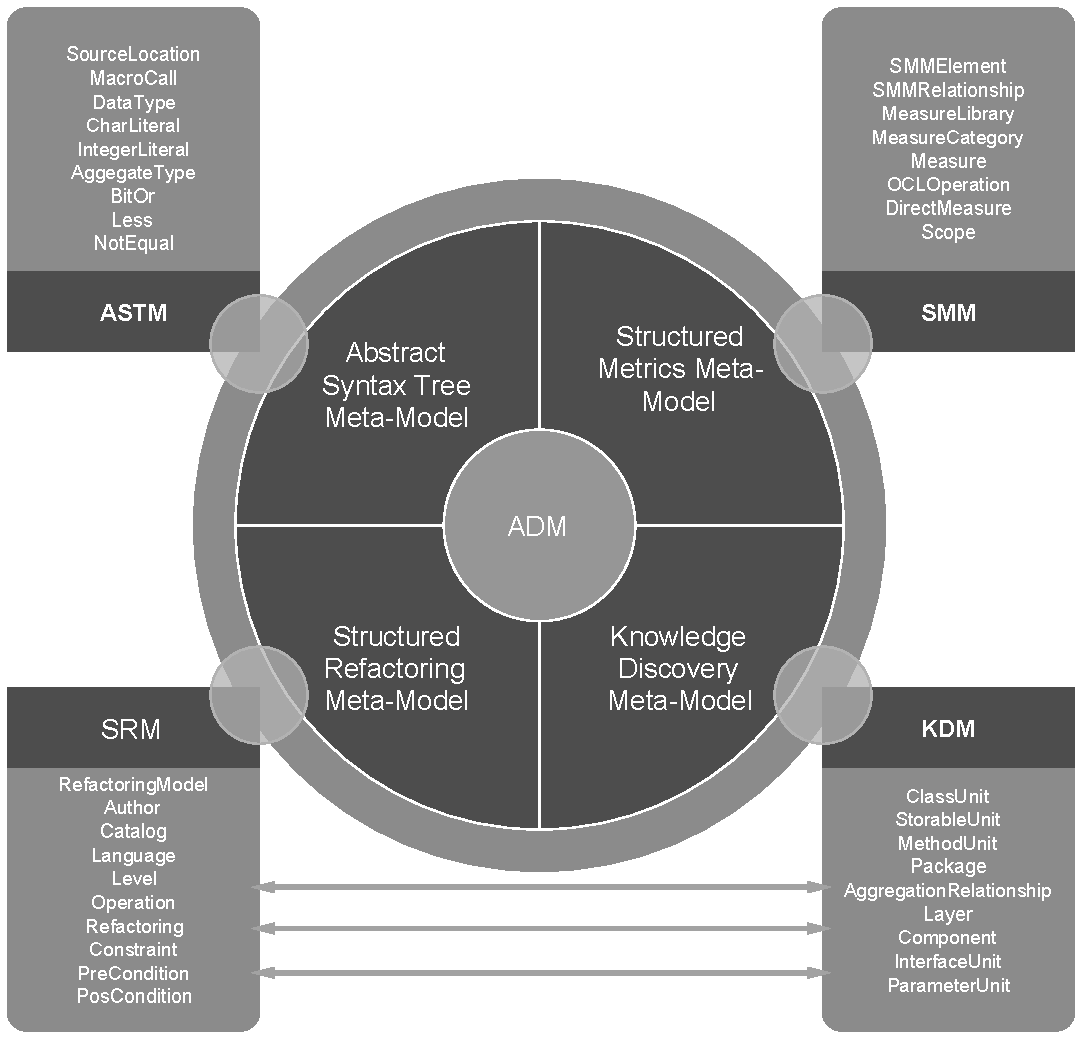
\includegraphics[scale=0.65]{images/SRM2Formatted}
	\fautor
\end{figure}

Como pôde ser observado na Figura~\ref{fig:refactoring_metamodel} o SRM está inserido no contexto da ADM para preencher a definição de um metamodelo de refatorações. Um dos objetivos do SRM é seguir as padronizações propostas pela ADM. Porém, deve-se ressaltar que o SRM é utilizado para especificar a representação de refatorações sem se preocupar com a representação das partes estruturais de uma refatoração, ou seja, os elementos que serão refatorados (classes, métodos, atributos, etc.). Assim, o SRM assume que tais elementos (classes, métodos, atributos, etc.) devem ser representados utilizando outro metamodelo proposto pela ADM, como, por exemplo, o KDM. Como visualizado na Figura~\ref{fig:refactoring_metamodel}, o SRM iterage com o metamodelo KDM, ou seja, o SRM utiliza instâncias de metaclasses do KDM para a aplicação da operação/mecanismo de uma refatoração propriamente dita.

Consistente com outros metamodelos definidos pela OMG, o SRM é definido utilizando a padronização  de modelagem MOF e a \textit{framework} EMF. Um dos benefícios de utilizar MOF é que o mesmo permite que o metamodelo seja serializado e deserializado sem perder nenhum tipo de informação, ou seja, metamodelos instanciados são representados utilizando uma representação textual padronizada, XMI. Além disso, o SRM é compatível com repositórios MOF para armazenamento e recuperação de várias ferramentas, aumentando assim a interoperabilidade de futuras ferramentas que utilizem esse metamodelo.

\section{Fases para a Construção e Uso do SRM}\label{abordagem_para_a_construcao_e_uso_do_SRM}

As construção e uso do SRM é composta de duas principais fases, Engenharia do SRM e Engenharia da Refatoração, como mostrado na Figura~\ref{fig:fases_para_a_construcao_e_uso_do_SRM}. A notação de \sigla{SADT}{\textit{Structured Analysis and Design Technique}}~\cite{Marca_1987} é utilizada na Figura~\ref{fig:fases_para_a_construcao_e_uso_do_SRM}.

\begin{figure}[h]
	\centering
	% Requires \usepackage{graphicx}
	\caption{Fases para a construção e uso do SRM.}
	\label{fig:fases_para_a_construcao_e_uso_do_SRM}
	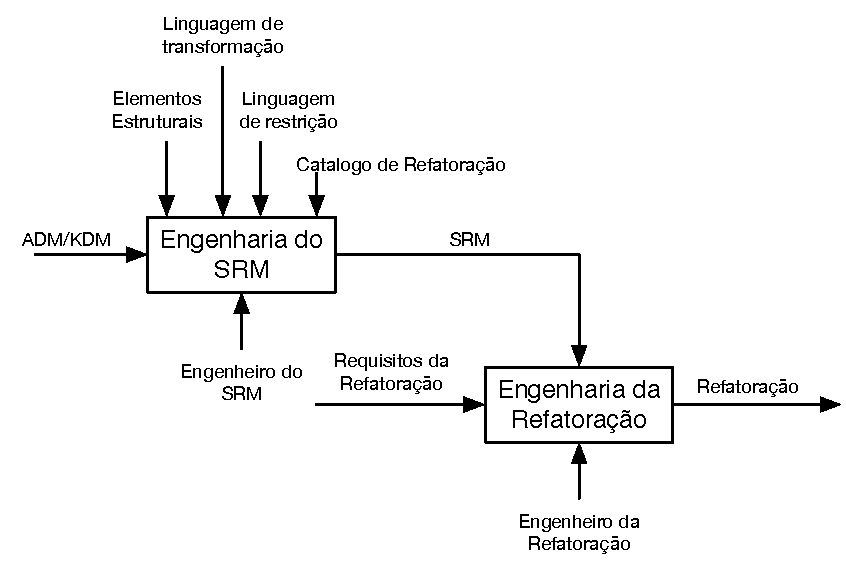
\includegraphics[scale=0.9]{images/fasesParaConstruirOSRM}
	\fautor
\end{figure}

A fase A, Engenharia do SRM, apresentada em detalhes na Seção~\ref{Engenharia_do_Meta_modelo_SRM}, tem como entrada um conjunto de elementos que foram utilizados como base para o desenvolvimento do SRM. Nesta fase o Engenheiro do SRM faz uso de elementos estruturais, linguagens de transformações, linguagens de restrições e catálogos de refatorações para desenvolver o SRM.

%Na fase de Engenharia da Refatoração, apresentada em detalhes na Seção X, a meta-linguagem XText\footnote{https://eclipse.org/Xtext/} foi utilizada para a criação de uma DSL. Essa DSL tem como objetivo principal diminuir quantidade de código-fonte, esforço obrigatórios e competência necessárias para instanciar refatorações utilizando o SRM.

%Na fase de Engenharia do Repositório, apresentada em detalhes na Seção X, um repositório, bem como uma aplicação web foram desenvolvidas para auxiliar o compartilhamento de refatorações utilizando o metamodelo SRM.

Finalmente, na fase Engenharia da Refatoração, é apresentado como o metamodelo SRM é instanciado utilizando uma DSL e/ou uma aplicação \textit{web}. Em seguida é apresentado como uma refatoração instanciada utilizando o metamodelo SRM pode ser compartilhado utilizando o repositório. Ainda nessa fase é ilustrado como uma refatoração é aplicada em uma instancia do KDM.

\subsection{Engenharia do SRM}\label{Engenharia_do_Meta_modelo_SRM}

Na fase de Engenharia do SRM, refatorações e suas características em geral são analisadas para que o SRM seja projetado e implementado. As oito etapas que compõem essa fase são mostradas na Figura~\ref{fig:etapas_da_fase_de_e_do_SRM}: (\textit{i}) Identificação dos Elementos Estruturais, (\textit{ii}) Identificação das Linguagens de Transformações, (\textit{iii}) Identificação das Linguagens de Restrições, (\textit{iv}) Identificação de vocabulário; (\textit{v}) Projeto do SRM; (\textit{vi}) Construção do SRM; (\textit{vii}) Construção da DSL, e (\textit{viii}) Construção do Repositório. 

\begin{figure}[h]
	\centering
	% Requires \usepackage{graphicx}
	\caption{Etapas da fase de Engenharia do SRM.}
	\label{fig:etapas_da_fase_de_e_do_SRM}
	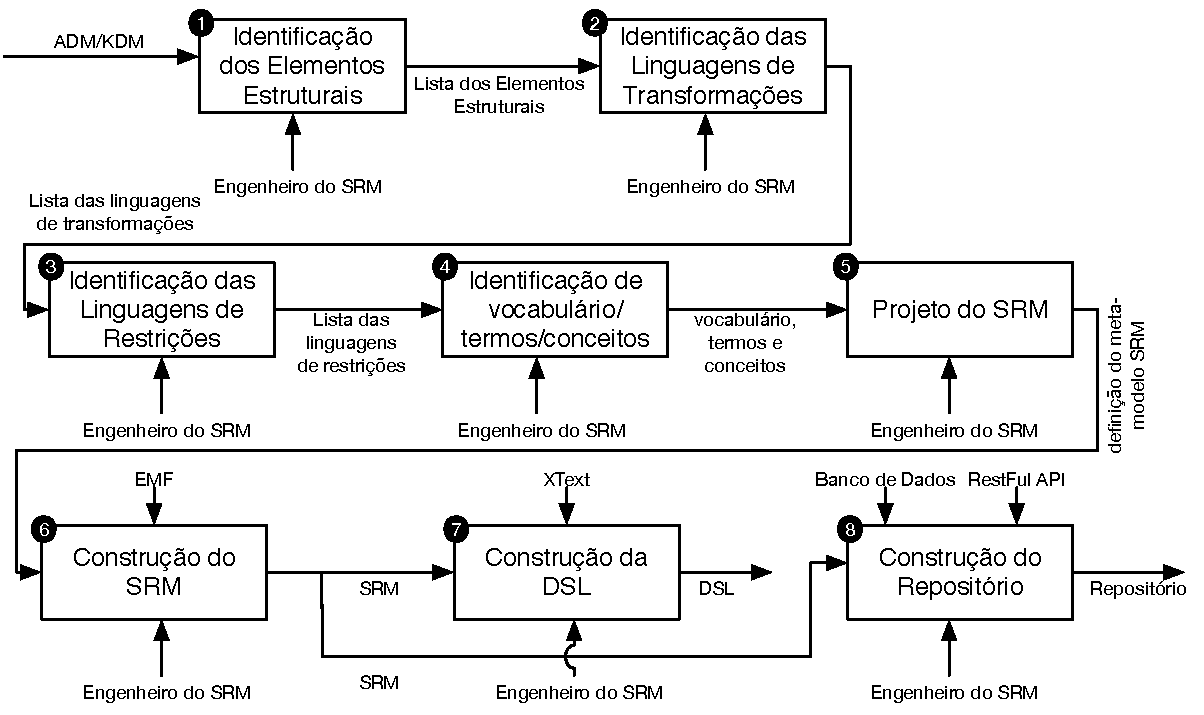
\includegraphics[scale=0.75]{images/todasAsFasesDaEngenhariaDOSRM5}
	\fautor
\end{figure}

\subsubsection{Identificação dos Elementos Estruturais}
%quatro principais elementos foram utilizados para auxiliar o desenvolvimento do SRM. Tais elementos são apresentados na Figura 2 e são descritos a seguir.

%\begin{enumerate}
%\item Elementos estruturais;
%\item Linguagem de transformação;
%\item Linguagem de restrição; e
%\item Catalogo de refatoração.
%\end{enumerate}
Esta etapa possui como objetivo analisar e identificar possíveis elementos estruturais para serem utilizados durante a refatoração. No Capítulo~\ref{chapter:catalogo_refactoring_KDM} Seção~\ref{sec:mapeamento_POO_e_KDM}, a Tabela~\ref{tab:mapemanetoEntreOOPeKDM} apresenta uma relação existente entre os conceitos do POO, bem como algumas instruções de linguagens de programção e o metamodelo KDM. Para fazer com o que o metamodelo SRM seja independente de linguagem e plataforma foi utilizado os elementos (metaclasses) do KDM para representar os elementos estruturais. Como já salientado no Capítulo~\ref{chapter:catalogo_refactoring_KDM}, o metamodelo KDM contêm algumas metaclasses que podem ser diretamente mapeadas a elementos estruturais, tal como, classes (\texttt{ClassUnit}), interfaces (\texttt{InterfaceUnit}), atributos (\texttt{StorableUnit}), métodos (\texttt{MethodUnit}), etc. Essas metaclasses possuem o mesmo objetivo e características dentro do contexto do POO e linguagens de programação. Entretanto, como o KDM tem como objetivo ser um modelo independente de plataforma, ou seja, tem como intuito representar de forma genérica todas as abstrações e paradigmas de programação, algumas construções de programação não possuem uma metaclasse particular. Por exemplo, iterações e ramificações em KDM são representadas utilizando a mesma metaclasse, \texttt{ActionElement}.

Neste contexto, elementos estruturais no contexto deste capítulo representam as instâncias das metaclasses que serão refatorados, por exemplo, \texttt{ClassUnit}, \texttt{MethodUnit}, \texttt{StorableUnit}, etc. Tais metaclasses foram consideradas boas candidatas para facilitar o reuso e troca de metadados no metamodelo SRM. Por exemplo, considere a refatoração \textit{RenameX}, onde \textit{X} pode ser qualquer elemento estrutural (\texttt{ClassUnit}, \texttt{MethodUnit}, \texttt{StorableUnit}, etc.). Os passos e mecanismo necessários para realizar essa refatoração são iguais ou possuem poucas diferenças não importa o tipo de elemento que será refatorado. Tendo como base esse exemplo, é possível identificar a necessidade de representar os metadados dos elementos estruturais que serão refatorados no SRM. Como o KDM (ver Capítulo~\ref{chapter:adm_kdm}) foi desenvolvido com o intuito de representar todo o sistema, bem como, seus artefatos – o mesmo é um bom candidato para representar os elementos estruturais de uma refatoração. Assim, nesta etapa as metaclasses do metamodelo KDM foram consideradas boas candidatas para serem os elementos estruturais das refatorações.

\subsubsection{Identificação das Linguagens de Transformações}

Nesta etapa são identificadas e analisados os detalhas de um conjunto de linguagens de transformações com o intuito de identificar as informações necessários para promover o reuso do mecanismo das refatorações. 

Conceitualmente, refatorações são definidas por meio de um conjunto de passos que devem ser seguidos para realizar uma determina mudança~\cite{Fowler1999, Demeyer1}. Por outro lado, programaticamente as refatorações são definidos como \aspas{programas} parametrizados que executam um conjunto de transformações seguindo uma ordem lógica. Usualmente, no contexto de modelos, tais transformações são conhecidas como endógenas e são implementadas utilizando técnicas de reescrita de grafo, ou como também é conhecida transformação de grafo (ver Capítulo~\ref{chapter:fundamentacao_teorica} Seção~\ref{sec:transformacoes_de_modelos}). Dessa forma, pode-se caracterizar que técnica de reescrita de grafo é útil para auxiliar na elaboração de transformações de forma independente para \textit{n} metamodelos, ou seja, técnica de reescrita de grafo pode ser aplicada em qualquer metamodelo que implemente o padrão MOF, como por exemplo o metamodelo KDM. 

Comumente, transformações em modelos são definidas utilizando linguagens específicas de transformações de modelos. Diversas linguagens de transformação de modelos têm sido propostas atualmente~\cite{Biehl_2010, Allilaire_06}, entre elas pode-se citar ATL e QVT. Por exemplo, no Código-fonte~\ref{codigo:rename_classUnit_SRM} é apresentado um trecho da refatoração \texttt{Rename ClassUnit} escrito em ATL. Nota-se que utilizando a linguagem de programação ATL facilmente pode-se especificar qual metamodelo esta sendo utilizado na refatoração. Além disso, com o uso da ATL e QVT pode-se automatizar os mecanismos e todos os passos que uma determinada refatoração deve realizar. Por exemplo, no Código-fonte~\ref{codigo:rename_classUnit_SRM} uma determinada instância de \texttt{ClassUnit} que contêm o meta-atributo \texttt{name} igual à \aspas{Fusca} será refatorada para \aspas{Ferrari}. Dessa forma, com o propósito de automatizar os mecanismo e todos os passos de uma refatoração no contexto do metamodelo SRM, tanto ATL e QVT foram considerados bons candidatos para especificar programaticamente o metadados sobre refatorações. ATL e QVT foram escolhidas como linguagens de transformação nesta capítulo considerando vários aspectos. Tais linguagens estão integradas na plataforma Eclipse, o que fornece uma série de recursos padrões para o desenvolvimento (\textit{syntax highlighting} e \textit{debugger}). Ambas linguagens são parte do projeto \textit{Model-To-Model} e possuem um grupo de discussão ativo, constantemente atualizado, vários exemplos e diversos estudos de casos aplicados até mesmo na indústria utilizam tais linguagens.


\begin{codigo}[caption={[Refatoração \textit{Rename ClassUnit}.] Refatoração \textit{Rename ClassUnit}.},escapeinside={(*@}{@*)}, basicstyle=\footnotesize, label={codigo:rename_classUnit_SRM}, language=ATL]{Name}
module renameClassUnit;
create OUT : MM refining IN : MM;
rule renameClassUnit {
	from
		source : MM!ClassUnit (source.name = (*@\aspas{Fusca}@*))
	to 
		target : MM!ClassUnit (
			name (*@$\leftarrow$@*) (*@\aspas{Ferrari}@*)
		)
}
\end{codigo}



%Linguagem de transformação representam as operações/mecanismos de um refatoração. Tais operações/mecanismos são responsáveis por realizar a refatoração propriamente dita no metamodelo. Usualmente  tais transformações são escritas em linguagens imperativas como \textit{Query}/\textit{View}/-\textit{Transformation} (QVT) ou ATL \textit{Transformation Language}.

\subsubsection{Identificação das Linguagens de Restrições}
Nesta etapa as formas de especificar as restrições são identificadas para definir as pré- e pós-condições de uma determinada refatoração. É importante que o metamodelo SRM permita definir tais restrições e não apenas o mecanismo da refatoração, assim, engenheiros podem utilizar uma determinada instância do metamodelo SRM e verificar quais são as restrições que eles devem respeitar para executar a refatoração de forma correta. 

Por exemplo, usualmente antes e depois de executar o mecanismo de uma determinada refatoração algumas restrições precisam ser satisfeitas. Tais restrições usualmente são úteis para verificar se os parâmetros necessários para executar a refatoração foi completamente e corretamente informando, bem como verificar se a refatoração foi aplicada de forma totalmente correta. No contexto de modelos, tais restrições são especificadas utilizando linguagens como OCL e XQuery. Tais restrições no contexto de refatorações são conhecidas como pré- e pós-condições. Utilizando tais linguagens, é possível verificar, por exemplo, se todos os parâmetros obrigatórios para executar o mecanismo da refatoração foram especificados pelo modernizador. Além disso, essas condições são importantes para assegurar que a refatoração será aplicada de forma correta e ainda irá preservar a semântica da instância do metamodelo, como por exemplo, preservar comportamentos, sincronização, etc. 

Com o propósito de automatizar as pré- e pós-condições de uma refatoração no contexto do metamodelo SRM, tanto OCL e XQuery foram considerados bons candidatos para especificar programaticamente as restrições que devem ser satisfeitas e respeitadas para a execução da refatoração.

%Condições prévias de refatoração são propriedades do programa original que deve segurar por um refactoring ser de preservação comportamento.


%Linguagem de restrição no contexto desse capítulo representa pré- e pós-condição de uma refatoração. Usualmente no contexto de modelos, restrições podem ser escritas utilizando a \textit{Object Constraint Language} (OCL).

\subsubsection{Identificação de vocabulário/termos/conceitos}

Nesta etapa é realizada a identificação de vocabulário, termos e conceitos comuns que são utilizadas dentro da comunidade de refatoração. Durante a criação de metamodelos é de suma importância entender o domínio que o metamodelo representa. metamodelos definem abstrações (termos), notações e relacionamentos para representar um determinado domínio. Assim, nesta etapa tanto os vocabulários, termos e conceitos definidos por~\citeonline{OPDYKE_1992} e \citeonline{Fowler1999} foram analisados para a identificação de abstrações para facilitar a criação do metamodelo SRM. Durante a análise pode-se observar e identificar alguns termos comumente utilizados durante a definição de uma refatoração. Por exemplo, todas as refatorações descritas e definidas por~\citeonline{OPDYKE_1992} e \citeonline{Fowler1999} seguem os seguintes termos: 

\begin{itemize}
\item Autor: autor da refatoração;
\item Catalogo: o catalogo no qual a refatoração pertence;
\item Biblioteca de refatoração: onde um conjunto de catálogos podem ser incluidos;
\item Nome: o nome da refatoração;
\item Descrição: informando uma típica situação onde a refatoração deveria ser aplicada;
\item Motivação: informando a motivação para a realização da refatoração;
\item Operação: descrevendo os passos que devem ser realizados para executar a refatoração;
\item Parâmetros: informações necessários para executar a operação da refatoração;
\item Restrições: pré- e pós-condições informando as restrições que devem ser safisfeitas durante e após a realização da refatoração.
\end{itemize}

\subsubsection{Projeto do SRM}

Nesta etapa o SRM é especificado a partir das informações extraídas nas etapas anteriores. Utilizando as informações extraídas foi possível identificar terminologias, bem como palavras chaves que geralmente estão relacionadas com refatoração. Utilizando tais terminologias e palavras chaves foi possível realizar a especificação do SRM. O SRM pode ser definido como uma quadrupla, como observado na Definição~\ref{def:SRM}: 


\begin{definicao}\label{def:SRM}
    \textit{O SRM é uma quadrupla $SRM = (SRM_{mC}, SRM_{mA}, SRM_{e}, SRM_{mR})$ onde $SRM_{mC} $ representa um conjunto de metaclasses, $SRM_{mA}$ representa um conjunto de meta-atributos, $SRM_{e}$ representa um conjunto de enumerações e $SRM_{mR}$ representa associações.}
\end{definicao}

Formalmente pode-se definir o metamodelo como:

\begin{itemize}
	\item Todas as metaclasses \textit{mC} $\in SRM_{mC}$ tem um nome que representa o seu significado;
	\item Todos os meta-atributos \textit{mA} $\in SRM_{mA}$ contêm um nome, um tipo e uma cardinalidade. Além disso, cada mA está associado a uma metaclasse;
	\item Todas as enumerações \textit{e} $\in SRM_{mA}$ contêm um nome e um valor;
	\item Todas as meta-associações \textit{mR} $\in SRM_{mR}$ é um conjunto R = $E_{1}$, $E_{2}$  , onde  $E_{1}$ e $E_{2}$ são chamadas de association ends de R. Posteriormente, cada R, contêm um nome. Ambos $E_{1}$  e $E_{1}$ possuem uma cardinalidade e são associados a uma metaclasse de $SRM_{mC}$.
\end{itemize}

Na Figura~\ref{fig:meta_modelo_SRM} é apresentado o metamodelo SRM. O SRM contêm 12 metaclasses e três enumerações. Esse metamodelo foi desenvolvimento utilizando o EMF. Um descrição detalhada de cada elementos desse metamodelo é apresentado a  seguir:

\begin{figure}[h]
	\centering
	% Requires \usepackage{graphicx}
	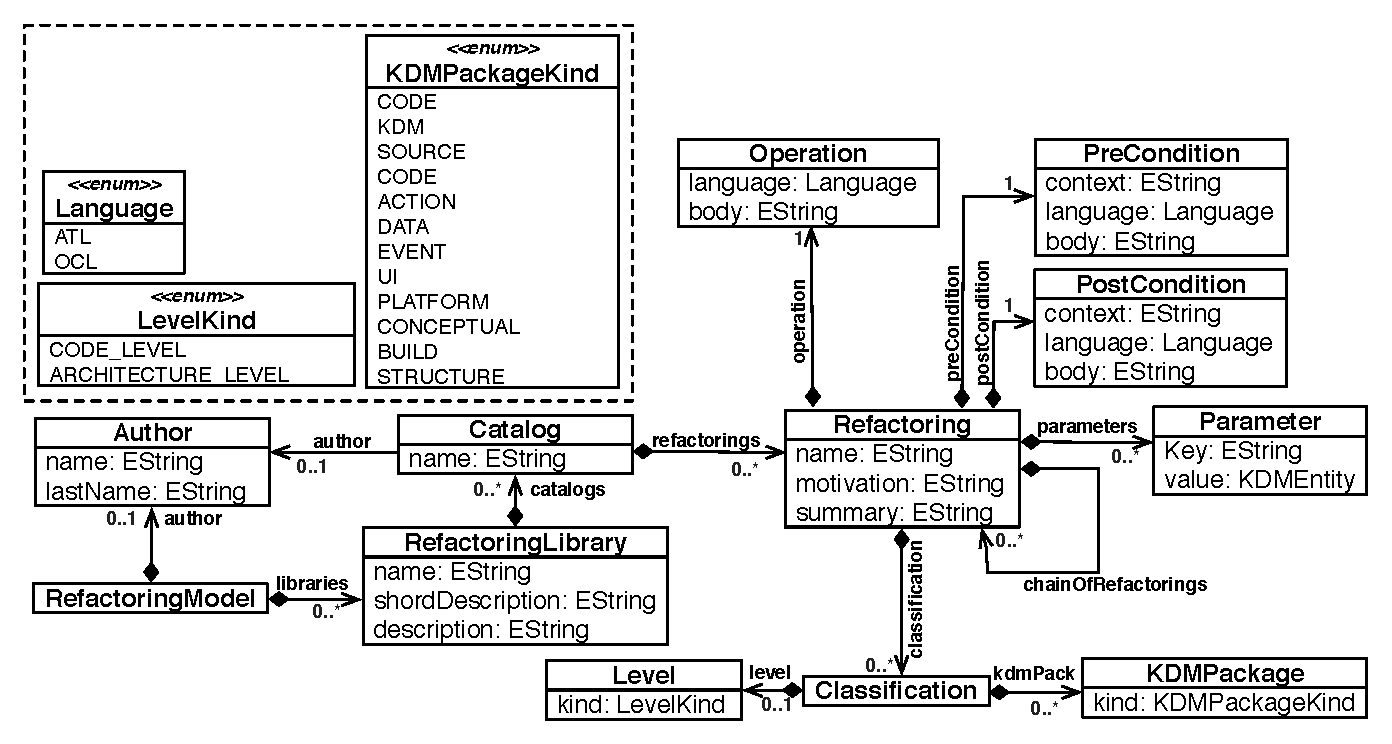
\includegraphics[scale=0.65]{images/refactoring_metamodel}
	\caption{metamodelo SRM.}
	\label{fig:meta_modelo_SRM}
\end{figure}

\begin{itemize}
\item \texttt{RefactoringModel} representa a metaclasse raiz do metamodelo.

\begin{itemize}
	\item \textbf{Associações}
		\begin{itemize}
			\item \texttt{author:Author[0..1]}: representa o autor de uma refatoração; 
			\item \texttt{libraries:RefactoringLibrary[0..*]}: representa um conjunto de biblioteca de refatorações que uma instância da metaclasse \texttt{RefactoringModel} possui..
		\end{itemize}
\end{itemize}

\item \texttt{Author} representa o autor de uma refatoração. Essa metaclasse contêm dois meta-atributos.

\begin{itemize}
	\item \textbf{Meta-atributos}
		\begin{itemize}
			\item \texttt{name}: utilizado para definir o nome do autor;
			\item \texttt{lastName}: utilizado para definir o sobrenome do autor.
		\end{itemize}	
\end{itemize} 

\item \texttt{RefactoringLibrary} utilizado para descrever uma biblioteca de refatorações.

\begin{itemize}
	\item \textbf{Attributes}
		\begin{itemize}
			\item \texttt{name}: utilizado para descrever o nome da biblioteca de refatoração;
			\item \texttt{shortDescription}: representa uma breve descrição sobre a biblioteca de refatoração;
			\item \texttt{description}: representa uma completa descrição sobre a biblioteca de refatoração.
		\end{itemize}	
\end{itemize} 

\begin{itemize}
	\item \textbf{Associação}
		\begin{itemize}
			\item \texttt{catalogs:Catalog[0..*]}: um conjunto de catálogos que contem refatorações.
		\end{itemize}	
\end{itemize} 

\item \texttt{Catalog} metaclasse utilizada para representar um catalogo de refatorações.

\begin{itemize}
	\item \textbf{Meta-atributos}
		\begin{itemize}
			\item \texttt{name}: representa o nome do catálogo. 
		\end{itemize}	
\end{itemize} 

\begin{itemize}
	\item \textbf{Associações}
		\begin{itemize}
			\item \texttt{author:Author[0..1]}: representa o autor do catalogo;
			\item \texttt{refactorings:Refactoring[0..*]}: conjunto de todas as refatorações que um catalogo contêm.
		\end{itemize}	
\end{itemize} 

\item \texttt{Refactoring} representa uma das principais metaclasses do SRM.

\begin{itemize}
	\item \textbf{Meta-atributos}
		\begin{itemize}
			\item \texttt{name}: utilizado para identificar a refatoração e ajuda a construir um vocabulário comum para os desenvolvedores de software;
			\item \texttt{motivation}: descreve o motivo pelo qual a refatoração deve ser realizada – lista também as circunstâncias na qual a refatoração deve ser utilizada;
			\item \texttt{summary}: informa quando e onde uma determinada refatoração deve ser utilizada. Também é útil para auxiliar o engenheiro de software a identificar uma refatoração relevante em uma determinada situação. 
		\end{itemize}	
\end{itemize} 

\begin{itemize}
	\item \textbf{Associações}
		\begin{itemize}
			\item \texttt{operation:Operation[1]}: deve a ação que será executa, representa o mecanismo da refatoração;
			\item \texttt{preCondition:PreCondition[1]}: representa uma pré-condição que deve ser satisfeita antes da execução da operação/refatoração;
			\item \texttt{postCondition:PostCondition[1]}: representa uma pós-condição que tem como intuito verificar a corretude da refatoração;
			\item \texttt{parameters:Parameter[0..*]}: um conjunto de parâmetros que são utilizados para realizar a refatoração. Tais parâmetros podem ser metaclasses do KDM;
			\item \texttt{chainOfRefactoring:Refactoring[0..*]}: um conjunto de refatorações que quando combinados podem realizar refatorações complexas, ou seja, \textit{macro-grained refactoring};
			\item \texttt{classification:Classification[0..*]}: define a classificação de uma refatoração.
		\end{itemize}	
\end{itemize} 

\item \texttt{Operation} também representa uma das principais metaclasses do SRM. Essa metaclasse contêm metadados do código responsável por realizar a transformação/refatoração.

\begin{itemize}
	\item \textbf{Meta-atributos}
		\begin{itemize}
			\item \texttt{language}: especifica a linguagem que será escrito o código responsável por realizar a transformação/refatoração. Valores válidos são: ``ATL'' e ``QVT'';
			\item \texttt{body}: especifica a transformação/refatoração com base na linguagem selecionada, ``ATL'' ou ``QVT''.
		\end{itemize}	
\end{itemize} 

\item \texttt{PreCondition} define uma pré-condição para ser executada antes de operação/refatoração.

\begin{itemize}
	\item \textbf{Meta-atributos}
		\begin{itemize}
			\item \texttt{context}: especifica o classificador para qual a pré-condição será definido;
			\item \texttt{language}: especifica a linguagem que será escrito a pré-condição. Valor válido é: ``OCL'' ou ``XQuery'';
			\item \texttt{body}: especifica a OCL ou ``XQuery'' que representa a pré-condição.
		\end{itemize}	
\end{itemize} 

\item \texttt{PostCondition} define uma pós-condição para ser executada após a operação/refatoração.

\begin{itemize}
	\item \textbf{Meta-atributos}
		\begin{itemize}
			\item \texttt{context}: especifica o classificador para qual a pós-condição será definido;
			\item \texttt{language}: especifica a linguagem que será escrito a pós-condição. Valor válido é: ``OCL'' ou ``XQuery'';
			\item \texttt{body}: especifica a OCL ou ``XQuery'' que representa a pós-condição.
		\end{itemize}	
\end{itemize} 

\item \texttt{Parameter} define um conjunto de parâmetros necessários para executar a refatoração. Essa metaclasse utiliza uma estrutura similar a tabela \textit{hash} para definir os parâmetros.

\begin{itemize}
	\item \textbf{Meta-atributos}
		\begin{itemize}
			\item \texttt{key}: representa o nome do parâmetro;
			\item \texttt{value}: representa o tipo do parâmetro. Esse tipo deve ser tipos primitivos (\textit{int}, \textit{string}, \textit{double}, \textit{float}, etc.) ou metaclasses do metamodelo KDM.
		\end{itemize}	
\end{itemize} 

\item \texttt{Classification} define a classificação da refatoração.

\begin{itemize}
	\item \textbf{Associações}
		\begin{itemize}
			\item \texttt{level}: representa se a refatoração é fine ou macro grained refactoring;;
			\item \texttt{kdmPack}: define qual pacote do KDM é necessário para executar a refatoração..
		\end{itemize}	
\end{itemize} 

\item \texttt{Level} utilizado para definir se a refatoração é de granularidade baixa ou alta..

\begin{itemize}
	\item \textbf{Meta-atributos}
		\begin{itemize}
			\item \texttt{kind}: especifica o level da refatoração..
		\end{itemize}	
\end{itemize} 

\item \texttt{KDMPackage} define qual pacote do KDM é necessário para executar a refatoração.

\begin{itemize}
	\item \textbf{Meta-atributos}
		\begin{itemize}
			\item \texttt{kind}: representa qual pacote do KDM é necessário para executar a refatoração.
		\end{itemize}	
\end{itemize} 

\end{itemize}

Três enumerações também foram definidas, como pode ser observado na Figura~\ref{fig:meta_modelo_SRM} delimitada por um retângulo de linha pontilhada. A primeira enumeração é \texttt{Language}, que é utilizada para especificar a linguagem da operação/refatoração, valores válidos são: ``ATL'' e ``OCL''. A segunda enumeração é \texttt{LevelKind}, a qual é utilizada para definir o level da refatoração. Finalmente, \texttt{KDMPackageKind} é utilizado para definir qual pacote do metamodelo KDM é (são) utilizado(s) durante a execução da refatoração. 



\subsubsection{Construção da DSL}

Nesta etapa é realizado a construção de uma DSL para auxiliar o engenheiro durante a instanciação do metamodelo SRM. A fim de utilizar plenamente as vantagens dos metamodelo SRM, os engenheiros precisam ter um bom conhecimento de linguagem de programação avançada. Na verdade os desenvolvedores devem estar familiarizados como as semânticas das refatorações (por exemplo, qual(is) é (são) o(s) pré-requisito(s) para a execução de uma refatoração) e como/onde utilizar e programar tais refatorações. A instanciação de uma refatoração utilizando o SRM é bastante verbosa, complexa e propensa a erros, pois exige conhecimento avançadas de refatoração e habilidades de programação em relação a API Ecore, uma vez que o SRM foi desenvolvido utilizando o EMF. É importante salientar que o metamodelo SRM foi desenvolvido de uma forma para permitir a reutilização das metaclasses já definidas no metamodelo KDM. Dessa forma, elementos estruturais que são utilizados em uma refatoração são representados por metaclasses previamentes já definidas no metamodelo KDM, tais como: \texttt{ClassUnit}, \texttt{InterfaceUnit}, \texttt{Package}, \texttt{StorableUnit}, etc.


No Código-fonte~\ref{cod:instancia_do_SRM} é apresentado um trecho onde é feita a instanciação em memória de algumas metaclasses definidas no metamodelo SRM. Como pode ser observado nesse código-fonte a instanciação das metaclasses do metamodelo SRM é um processo verboso e propenso a erros, o engenheiro deve saber exatamente como utilizar a API do \textit{framework} EMF para realizar a instanciação de uma determinada metaclasse. Metaclasses são instanciadas em EMF utilizando o conceito de fabrica (em inglês - \textit{Factory}). Além disso, cada fabrica de metaclasses possui um método \texttt{createX}, onde X representa o nome da metaclasse do metamodelo. 
Por exemplo, como pode ser observado na linha 1 do Código-fonte~\ref{cod:instancia_do_SRM} uma instância da metaclasse \texttt{Author} é com a interface \texttt{RefactoringModelFactory} por meio do método \texttt{createAuthor()}. Em seguida, todos os meta-atributos da metaclasse \texttt{Author} devem ser especificados como apresentado nas linhas 2 e 3 do Código-fonte~\ref{cod:instancia_do_SRM}. Com o objetivo de diminuir a quantidade de código-fonte, esforço obrigatórios e competência necessárias para instanciar refatorações utilizando o metamodelo SRM, foi desenvolvido uma DSL que auxilia a instanciação de refatorações sistematicamente. Na parte superior a esquerda da Figura~\ref{fig:DSL_SRM} é possível visualizar o relacionamento entre a DSL criada e as metaclasses do metamodelo SRM.

\begin{codigo}[caption={[Instanciação do metamodelo SRM programaticamente.] Instanciação do metamodelo SRM.},escapeinside={(*@}{@*)}, basicstyle=\footnotesize, label={cod:instancia_do_SRM}, language=Java]{Name}
Author author = RefactoringModelFactory.eINSTANCE.createAuthor();
author.setName("Rafael");
author.setLastName("Durelli");
RefactoringModel rM = RefactoringModelFactory.eINSTANCE.createRefactoringModel();
rM.setAuthor(author);
RefactoringLibrary library = RefactoringModelFactory.eINSTANCE.createRefactoringLibrary();
lib.setName("Fowler's refactorings");
lib.setDescription("Contains some Fowler's refactorings such as ExtractClass, RenameElements, PushMethod, PushAttribute, etc.");
lib.setShortDescription("Fine grained Refactorings");
rM.getLibraries().add(lib);
Catalog cat = RefactoringModelFactory.eINSTANCE.createCatalog();
cat.setAuthor(author);
cat.setName("Fowler's catalog");
libr.getCatalogs().add(cat);
...
\end{codigo}

\begin{figure}[!h]
	\centering
	% Requires \usepackage{graphicx}
	\caption{DSL para auxiliar a instanciação do SRM.}
	\label{fig:DSL_SRM}
	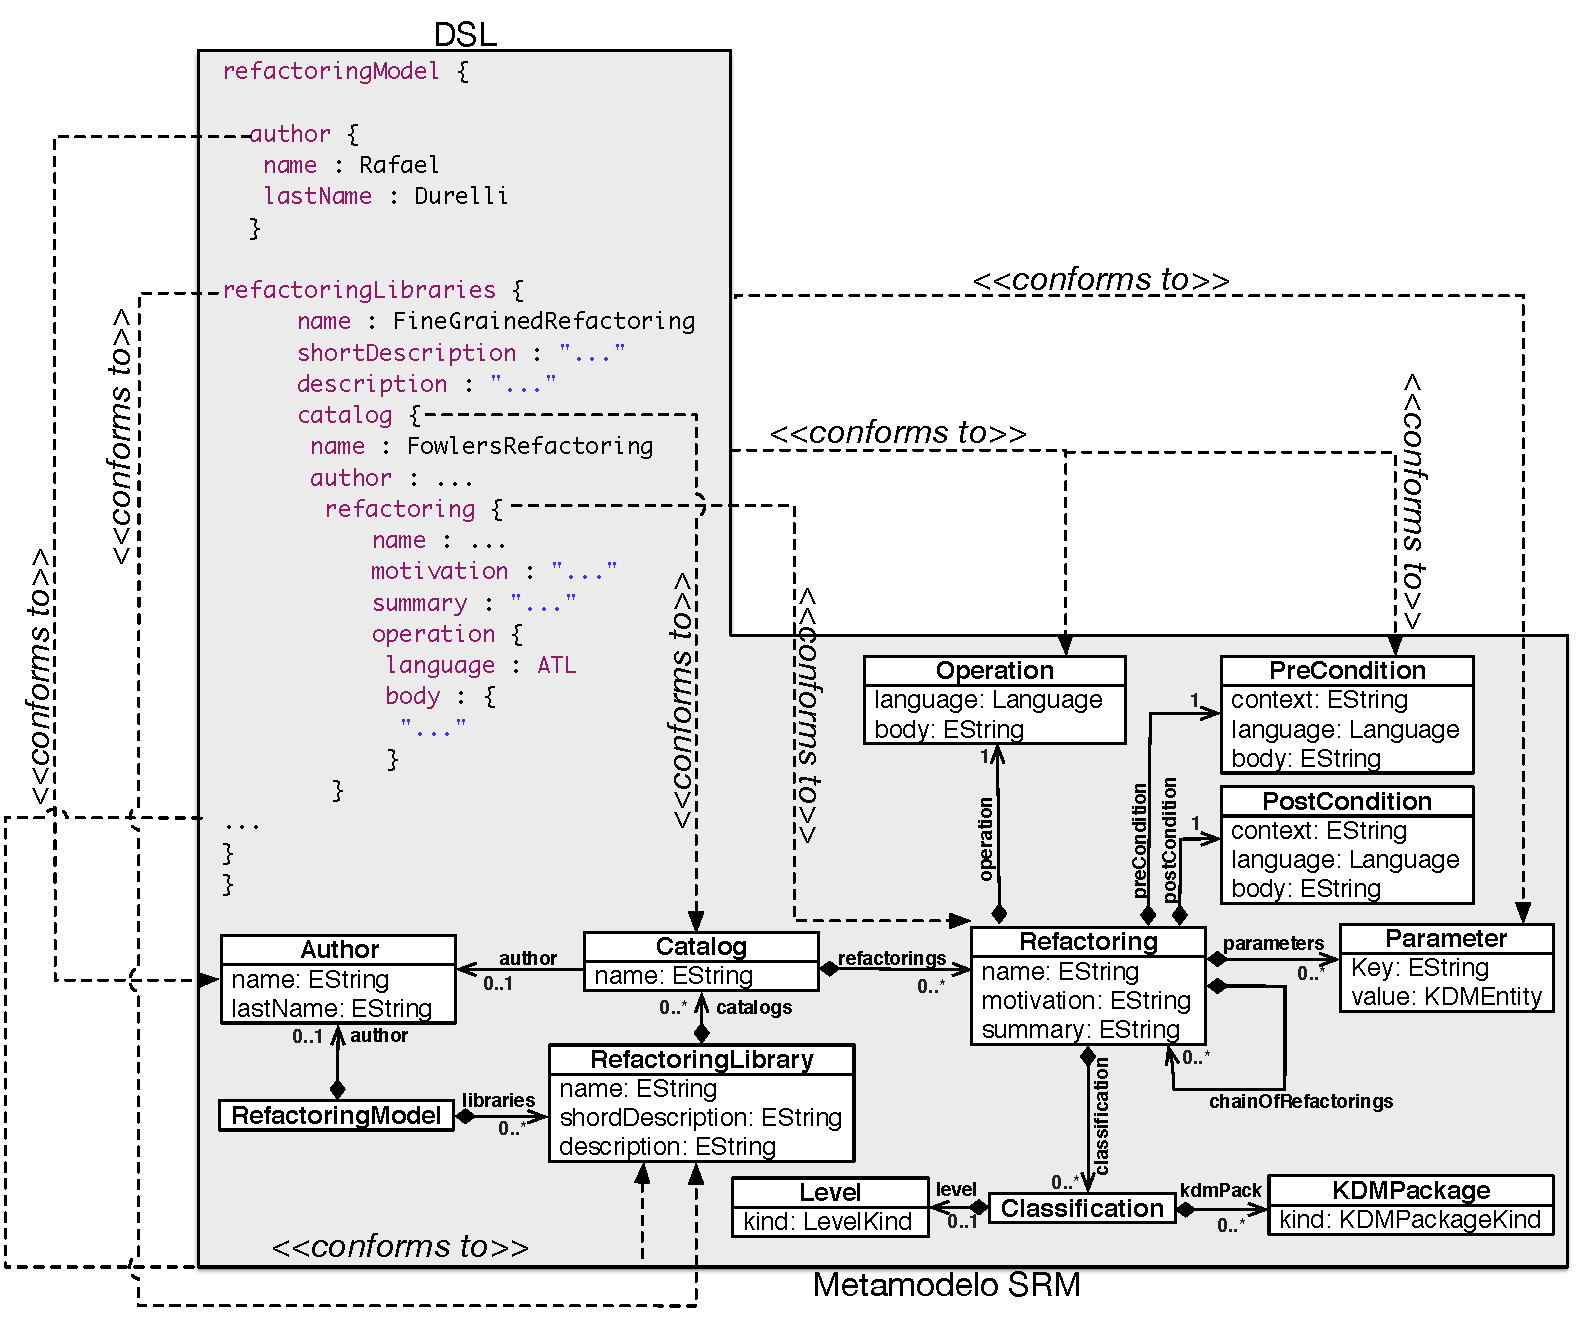
\includegraphics[scale=0.6]{images/MetaModelEDSL}
	\fautor
\end{figure}




A DSL criada para auxiliar a instanciação do SRM foi desenvolvida utilizando Xtext\footnote{\texttt{https://www.eclipse.org/Xtext/}}. Xtext é um \textit{framework} do Eclipse\footnote{\texttt{https://www.eclipse.org}} que facilita a definição de gramática\footnote{Gramáticas representam a definição formal de um sintaxe textual concreta. Consistem em um conjunto de regras de produção para definir como o \textit{textual input} (, ou seja,., sentenças) são representadas. Basicamente, as regras de produção podem ser representadas utilizando \textit{Backus–Naur Form} (BNF), por exemplo, \textit{S ::= P1 ... Pn}, essa gramática define um símbolo \textit{S} por um conjunto de expressões \textit{P1 ... Pn}.} 
com a utilização de um metamodelo que foi definido utilizando EMF. Xtext tem como principal objetivo automatizar e agilizar o processo de desenvolvimento de DSLs. Note que a sintaxe da DSL segue as terminologias e conceitos definidos no metamodelo SRM para facilitar a utilização da DSL e o entendimento do metamodelo SRM.

Em Xtext a gramática para especificar DSLs segue uma notação similar ao \textit{Backus–Naur Form} (BNF) chamada de regras do \textit{parser}. Tais regras representam a sintaxe concreta da DSL. Note que para facilitar o entendimento da DSL, trechos da mesma são mostradas em listagens de códigos separados, bem como símbolos para explanar o propósito de uma terminada linha da gramática. No Código-fonte~\ref{lst:dsl_part_1} é ilustrado o primeiro trecho da gramática concreta da DSL desenvolvida. 

\begin{lstlisting}[language=Xtext, frame=single, basicstyle={\scriptsize}, mathescape=true, label={lst:dsl_part_1}, caption={Gramática da DSL - parte 1}]
	
$\textrm{\ding{182}}$ grammar refactoring.xtext.SRM with org.eclipse.xtext.common.Terminals 
$\textrm{\ding{183}}$ import platform:/resource/refactoring/model/refactoringMetamodel.ecore
$\textrm{\ding{184}}$ import http://www.eclipse.org/emf/2002/Ecore as ecore
RefactoringModel: 
	$\textrm{\ding{185}}$ `refactoringModel' name = ID `{'
	$\textrm{\ding{186}}$ author = Author
	$\textrm{\ding{187}}$ libraries += RefactoringLibrary$^{*}$;
	`}'
\end{lstlisting}

A gramática começa com a definição do nome da DSL (SRM) (ver Código-fonte~\ref{lst:dsl_part_1} \ding{182}). Em sequência é definido os metamodelos que devem ser importados para serem utilizados durante a criação da DSL, ou seja, o metamodelo SRM\ding{183} e o Ecore\ding{184}.

Em seguida é criado a primeira regra. Essa regra começa com a definição da metaclasse \texttt{RefactoringModel}. O corpo da regra começa logo após os \aspas{\texttt{:}}. Primeiramente para o entendimento da regra, é importante destacar que literais de \textit{string} (que em Xtext podem ser expressas com aspas simples ou duplas) definem palavras-chave da DSL. Como pode ser observado no Código-fonte~\ref{lst:dsl_part_1} é esperado a palavra-chave \texttt{refactoringModel}\ding{185} seguido por um \texttt{ID} e ``\{''. A gramática que rege o objeto \texttt{ID} é definida como uma sequência ilimitada de maiúsculas e minúsculas, números e o carácter de sublinhado, embora possa não começa por um dígito. A gramática que representa o nó \texttt{ID}\ding{182} pode ser visualizada no Código-fonte~\ref{lst:dsl_part_2}. 

\begin{lstlisting}[language=Xtext, frame=single, basicstyle=\scriptsize, mathescape=true, label={lst:dsl_part_2}, caption={Gramática da DSL - parte 2}]
	$\textrm{\ding{182}}$ terminal ID: (`a'..`z' | `A'..`Z'|`_')(`a'..`z' | `A'..`Z'|`_'|`0'..`9')*;
\end{lstlisting}

Ainda no Código-fonte~\ref{lst:dsl_part_1} a expressão \texttt{author=Author}\ding{186} especifica que pode-se instanciar uma instancia da metaclasse \texttt{Author}. A expressão \texttt{(libraries += RefactoringLibrary)$^{*}$}\ding{187} descrita no Código-fonte~\ref{lst:dsl_part_1} especifica que pode-se instanciar várias instâncias da metaclasse \texttt{RefactoringLibrary}. O operador estrela, \aspas{\texttt{*}}, ilustra que o número de elementos (nesse caso \texttt{RefactoringLibrary}) é arbitrário; em particular, ele pode ser qualquer número \texttt{>=} 0. Operador \texttt{+=} por sua vez representa que a propriedade \texttt{libraries} será uma lista do tipo \texttt{RefactoringLibrary}.

\begin{lstlisting}[language=Xtext, frame=single, basicstyle=\scriptsize, mathescape=true, label={lst:dsl_part_3}, caption={Gramática da DSL - parte 3}]
Author:
	$\textrm{\ding{182}}$ `author' `{'
	$\textrm{\ding{183}}$ `name' `:' name = ID  
		$\textrm{\ding{229} \ding{184}}$ `lastName' `:' lastName = ID; 
`}'
RefactoringLibrary:
	$\textrm{\ding{185}}$ `refactoringLibraries' `{'
	$\textrm{\ding{186}}$ `name' `:' name = ID  
		$\textrm{\ding{229}}$ `shortDescription' `:' shortDescription = STRING
		$\textrm{\ding{229}}$ `description' `:' description = STRING
		$\textrm{\ding{229}}$ $\textrm{\ding{187}}$ catalogs += Catalog$^{*}$
`}'
\end{lstlisting}

A definição das regras que regem as metaclasses \texttt{Author} e \texttt{RefactoringLibrary} são apresentadas no Código-fonte~\ref{lst:dsl_part_3}. A regra para a definição de \texttt{Author} começa com a definição da palavra-chave \texttt{author} seguida por um `\{'\ding{182}. Em seguida a palavra-chave \texttt{name} é esperada, seguido por \aspas{\texttt{:}} \ding{183}. Posteriormente a palavra-chave \texttt{lastName} também é esperada, seguido por \aspas{\texttt{:}} \ding{184}. 

Na linha 6 do Código-fonte~\ref{lst:dsl_part_3} começa a definição da regra da metaclasse \texttt{RefactoringLibrary}. A regra para a definição de \texttt{RefactoringLibrary} começa com a definição da palavra-chave \texttt{refactoringLibraries} seguida por um `\{'\ding{185}. Em seguida, deve-se especificar a palavra-chave \texttt{name} e \texttt{:}. Posteriormente, as palavras-chaves \texttt{shortDescription} e \texttt{description} são especificadas nas linhas 9 e 10, respectivamente. A expressão descrita na Linha 11 representa que pode haver qualquer número de instâncias da metaclasse \texttt{Catalog}.

\begin{lstlisting}[language=Xtext, frame=single, basicstyle=\scriptsize, mathescape=true, label={lst:dsl_part_4}, caption={Gramática da DSL - parte 4}]
Catalog:
	$\textrm{\ding{182}}$`catalog' `{' 
		$\textrm{\ding{229} \ding{183}}$`name' `:' name=ID
		$\textrm{\ding{229} \ding{184}}$`author' `:' author=[Author]
		$\textrm{\ding{229} \ding{185}}$refactorings += Refactoring$^{*}$
	`}'
Refactoring:
	`refactoring' `{' 
		$\textrm{\ding{229}}$`name' `:' name = ID
		$\textrm{\ding{229}}$`motivation' `:' motivation = STRING
		$\textrm{\ding{229}}$`summary' `:' summary = STRING
		$\textrm{\ding{229} \ding{186}}$ operation = Operation?
		$\textrm{\ding{229} \ding{187}}$ preCondition = PreCondition?
		$\textrm{\ding{229} \ding{188}}$ postCondition = PostCondition?
		$\textrm{\ding{229} \ding{189}}$ classification = Classification
		$\textrm{\ding{229} \ding{190}}$(`containedRefactoring' `:' chainOfRefactoring+=Refactoring)$^{*}$
	`}'
\end{lstlisting}

O Código-fonte~\ref{lst:dsl_part_4} representa as sintaxes concretas das metaclasses \texttt{Catalog} e \texttt{Refactoring}, respectivamente. A sintaxe concreta da metaclasse \texttt{Catalog} começa com a palavra-chave \texttt{catalog} seguida por um `\{'\ding{182}. Em seguida o nome do catalogo de refatoração deve ser especifica por meio da palavra-chave \texttt{name} \ding{183}. Posteriormente, deve-se especificar uma instância da metaclasse \texttt{Author}, informando quem é o autor desse catalogo de refatoração, ver Código-fonte~\ref{lst:dsl_part_4}\ding{184}. Em seguida, na Linha 5 do Código-fonte~\ref{lst:dsl_part_4} deve-se informar várias instâncias da metaclasse \texttt{Refactoring}, essa sintaxe representa as refatorações que compõem esse catalogo de refatoração. Nas linhas 7-16 a definição da sintaxe concreta para a definição de uma refatoração por meio do metamodelo SRM é apresentada. Inicialmente, uma refatoração deve possuir um nome, conforme ilustrado na linha 9 do Código-fonte~\ref{lst:dsl_part_4}. Posteriormente, a motivação, bem como o resumo da refatoração também devem ser especificados, conforme apresentado nas linhas 10 e 11 do Código-fonte~\ref{lst:dsl_part_4}. As linhas 12, 13, 14 e 15 informam que uma metaclasse do tipo \texttt{Operation}\ding{186}, \texttt{PreCondition}\ding{187}, \texttt{PostCondition}\ding{188} e \texttt{Classification} \ding{189} devem ser instanciadas, respectivamente. Na linha 16 representa a sintaxe da DSL para especificar um conjunto de refatorações que quando combinadas podem realizar refatorações complexas.

No Código-fonte~\ref{lst:dsl_part_5} as sintaxes concretas das metaclasses \texttt{Operation}, \texttt{PreCondition} e \texttt{PostCondition} são definidas. Como observado a sintaxe concreta da metaclasse \texttt{Operation} inicia com a palavra-chave \texttt{operation} seguida por um `\{'\ding{182}. Em seguida, deve-se especificar qual a linguagem que a operação/refatoração será escrita. \texttt{Language} é uma enumeração (\textit{enum}) que está representado na linha 24 do Código-fonte~\ref{lst:dsl_part_5}. A linha 5 representa a sintaxe concreta para especificar o \aspas{corpo} da operação/refatoração propriamente dita \ding{184}. Na linha 8 a sintaxe concreta da metaclasse \texttt{PreCondition} é definida. Observe que a sintaxe concreta inicia com a palavra-chave \texttt{preCondition} seguida por um `\{'\ding{182}, \texttt{context}, \texttt{language} e \texttt{body}. A sintaxe concreta da metaclasse \texttt{PostCondition} é definida nas linhas 16 até 23. Note que a sintaxe é similar à sintaxe definida na metaclasse \texttt{PreCondition}.
\begin{lstlisting}[language=Xtext, frame=single, basicstyle=\scriptsize, mathescape=true, label={lst:dsl_part_5}, caption={Gramática da DSL - parte 5}]
Operation: 
	$\textrm{\ding{182}}$`operation' `{'
		$\textrm{\ding{229}}$`language' `:' language=Language
		`body' `:' `{'
			$\textrm{\ding{229} \ding{184}}$body = STRING
		`}'
	`}'
PreCondition: 
	$\textrm{\ding{185}}$`preCondition' `{'
		$\textrm{\ding{229}}$`context' `:' context=STRING
		$\textrm{\ding{229}}$`language' `:' language=Language
		`body' `:' `{' 
			$\textrm{\ding{229}}$body=STRING	
		`}'
	`}'
PostCondition: 
	$\textrm{\ding{186}}$`postCondition' `{'
		$\textrm{\ding{229}}$`context' `:' context=STRING
		$\textrm{\ding{229}}$`language' `:' language=Language
		`body' `:' `{' 
			$\textrm{\ding{229}}$body=STRING	
		`}'
	`}'
enum Language: 
	ATL | OCL | XQuery
\end{lstlisting}


\subsection{Construção do Repositório}

Para facilitar e promover o compartilhamento e o reuso das refatorações utilizando o metamodelo SRM é necessário uma forma que permita que modernizadores possam enviar e reutilizar refatorações instanciadas para um local central. Assim, outros modernizadores podem contribuir com a criação de um conjunto de metadados sobre refatorações para que outros modernizadores possam pesquisar, identificar e reutilizar refatorações em seu projeto durante a modernização. Dessa forma, nesta etapa um repositório foi criado para permitir a contribuição e reutilização de refatorações no contexto do SRM. 




\section{Considerações Finais}
\label{sec:consideracoes_finais}

